\documentclass[ ]{article}
\title{Revisão P2 \\ Divane Marcon}
\author{Erickson G. Müller}
\date{25 de Junho de 2024}

\usepackage[ ]{tikz}
\usepackage[ ]{pgfplots}
\usepackage[ ]{amsmath}
\usepackage[ ]{graphicx}

\begin{document}
\maketitle

\section{Conteúdos}
	\begin{enumerate}
		\item Derivadas
		\item Velocidade e Aceleração
		\item Integrais Definidas e Indefinidas
		\item Teorema Fundamental do Cálculo
		\item Cálculo de Áreas
	\end{enumerate}
\newpage

\section{Derivadas}
	A derivada é o coeficiente angular da reta tangente à curva f(x) num determinado ponto.\\
	
	\begin{minipage}{6 cm}
		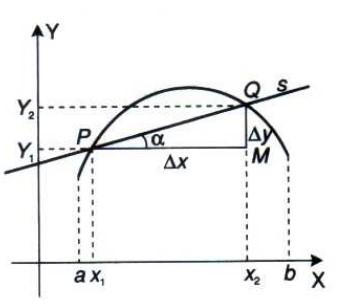
\includegraphics[scale=0.58]{Images/Graph1.jpg}
	\end{minipage}		
	\begin{minipage}{6 cm}
		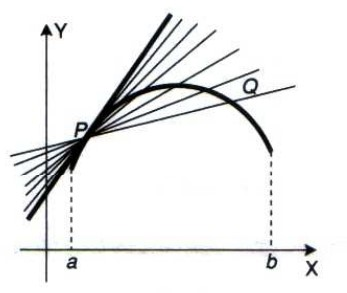
\includegraphics[scale=0.6]{Images/Graph2.jpg}
	\end{minipage}
	
	A curva tangente no ponto P	é calculada à medida que o ponto Q se aproxima do ponto P correndo sobre a curva.
	$$\lim_{Q_x\to P_x}f(x)=P'x+b$$
	Exemplo:\\
	Encontre a inclinação da reta tangente à curva $y=x^2-2x+1$ no ponto $(x_1,y_1)$.\\
	
	Se $f(x)=x^2-2x+1$, então $f(x)=x_1^2-2x_1+1$;\\
	$$f(x_1+\Delta x)=(x_1+\Delta x)^2 -2.(x_1+\Delta x) + 1$$
	$$=x_1^2+2.x_1.\Delta x + \Delta x^2 - 2.x_1 -2.\Delta x +1$$
	
	Usando limites...
	
	$$m(x_1) = \lim_{\Delta x \to 0}\dfrac{f(x_1+\Delta x)-f(x_1)}{\Delta x}$$
	$$=\lim_{\Delta x\to 0}\dfrac{x_1^2+2.x_1.\Delta x + \Delta x^2 - 2.x_1 -2.\Delta x +1 - (x_1^2-2x_1+1)}{\Delta x}$$
	$$=\lim_{\Delta x\to 0}\dfrac{2.x_1.\Delta x + \Delta x^2-2\Delta x}{\Delta x}$$
	$$ = \lim_{\Delta x\to 0}\dfrac{\Delta x.(2.x_1+\Delta x -2)}{\Delta x} = 2.x_1 - 2$$
	
	Por meio dessa derivação, provamos a propriedade de que $f'(x) = n.x^{n-1}$.
	\newpage
	Para entender melhor, irei desenhar um gráfico com as curvas $x^2-2x+1$ e $(2x-2).x+b$, para $x=3$:\\
	Ou seja, o $2x+b$ passa a ser o a da nova reta a ser descoberta, deste modo, se quisermos que a reta passe no ponto $(3,4)$, aplicaremos na fórmula da reta $y = ax+b$.
	$$4 = (2.3-2).3 + b$$
	$$a = 4$$ $$b=-8$$
	$$f'(x) = 4x - 8$$
	
	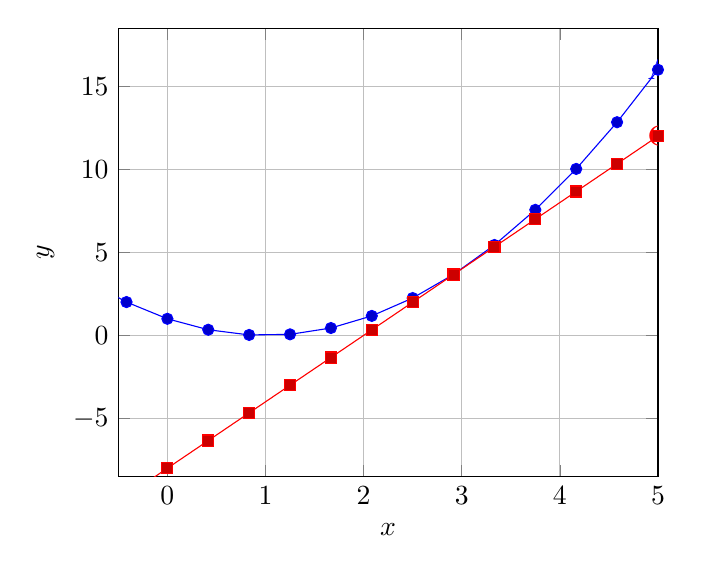
\begin{tikzpicture}
		\begin{axis}[
    		xlabel={$x$},
		    ylabel={$y$},
		    xmin = -0.5,  % Replace with your xmin value
		    xmax = 5,  % Replace with your xmax value
		    ymin = -8.5,  % This will be automatically calculated
		    ymax = 18.5,  % This will be automatically calculated
		    grid = major,]
		    
		    \addplot {x^2-2*x+1} node {A};
		    %\addplot {2*x-2} node {B};
		    \addplot {(2*3-2)*x - (2*3-2)*2} node {C};
		\end{axis}
	\end{tikzpicture}
	
	\subsection{Propriedades}
	
	\subsection{Derivada de ma Função num Ponto}
		A derivada da função $f(x)$ no ponto $x_1$, denotada por $f'(x_1)$, é definida pelo limite:
		
		$$f'(x) = \lim_{\Delta x\to 0} \dfrac{f(x_1+\Delta x)-f(x_1)}{\Delta x}$$
		ou
		$$f'(x) = \lim_{x_f\to x_0}\dfrac{f(x_f)-f(x_0)}{x_f-x_0}$$		
	\subsection{Velocidade e Aceleração}
		Existem dois tipos de cálculo para encontrar uma velocidade ou aceleração, a velocidade ou aceleração instantâneas e a velocidade e aceleração intervalares. A intervalar é calculada fazendo a média da diferença entre as distâncias ou as velocidades em um determinado intervalo de tempo ($\frac{s(t+\Delta t)-s(t)}{\Delta t}$). Para calcularmos a velocidade em determinado momento, precisamos aplicar o limite das velocidades médias quando $\Delta t$ se aproxima de 0.
		
		$$v(\Delta t) = \frac{s(t+\Delta t)-s(t)}{\Delta t}$$
		$$v(t) =\lim_{\Delta t\to 0}\frac{s(t+\Delta t)-s(t)}{\Delta t}= s'(t)$$
		
		Para calcular a aceleração, em vez da velocidade, apenas se substituem na fórmula as variáveis distância(s) pelas variáveis velocidade(v). Assim como a velocidade é calculada pela variação de distância, a aceleração é calculada pela variação de velocidade.
		
	\subsection{Regra da Cadeia}
	\subsection{Derivada das Funções Elementares}
	\subsection{Derivada das Funções Trigonométricas}
\section{Integrais}
	\subsection{Integrais Definidas}
	\subsection{Integrais Indefinidas}
	\subsection{Teorema Fundamental do Cálculo}
\section{Cálculo de Áreas}
	
\end{document}